\documentclass{beamer}
\usepackage[latin1]{inputenc}
\usepackage{xcolor}
\usepackage{hyperref}
\usepackage{minted}
\usepackage{graphicx}
\usepackage{tikz}
\usetikzlibrary{fadings}

\usetheme{default}
\usecolortheme{default}

\title{COMP3320 Introduction to OpenGL}
\author{Alex Biddulph}
\institute{
    The University of Newcastle, Australia
    \and
    Based on the work provided at \url{www.learnopengl.com}
}
\date{Semester 2, 2019}

\begin{document}

\begin{frame}
\titlepage
\end{frame}

\begin{frame}[fragile]{Object Colour}
    \begin{itemize}
        \item The colour that an object reflects
        \item[]
        \begin{center}
            
\includegraphics[height=0.30\textheight]{images/light_reflection.png}
        \end{center}
        \item This can be simulated as a simple multiplication
\footnotesize{
\begin{minted}{glsl}
    vec3 light_colour  = vec3(1.0f, 1.0f, 1.0f);
    vec3 object_colour = vec3(1.0f, 0.5f, 0.31f);
    vec3 result        = light_colour * object_colour;
\end{minted}
}
    \end{itemize}
    \vfill{}
    {\footnotesize{Image sourced from \url{learnopengl.com/Lighting/Colors}}}
\end{frame}

\begin{frame}[fragile]{Basic Lighting}
    \begin{center}
        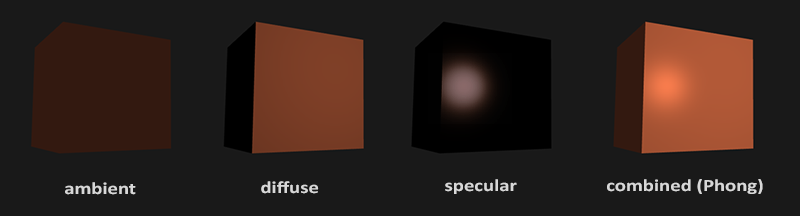
\includegraphics[height=0.30\textheight]{images/basic_lighting_phong.png}
    \end{center}
    \begin{center}
        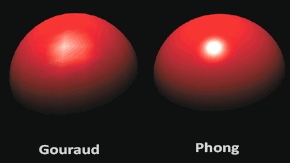
\includegraphics[height=0.30\textheight]{images/basic_lighting_gouruad.png}
    \end{center}
    \vfill{}
    {\footnotesize{Images sourced from \url{learnopengl.com/Lighting/Basic-Lighting}}}
\end{frame}

\begin{frame}[fragile]{Basic Lighting}
    \begin{itemize}
        \item Ambient: Background/global lighting. Results in objects being dimly lit when all 
            other lights are turned off.
        \item Diffuse: Brightness of reflected light is dictated by how closely the fragments 
            normal vector aligns with the light direction.
        \item Specular: Light is reflected about the fragments normal vector. Light appears 
            brightest when the viewing direction most closely aligns with the reflected direction.
        \begin{center}
            
\includegraphics[height=0.30\textheight]{images/diffuse_light.png}
            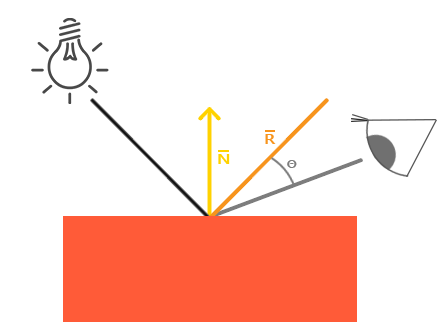
\includegraphics[height=0.30\textheight]{images/specular_light.png}
        \end{center}
    \end{itemize}
    \vfill{}
    {\footnotesize{Images sourced from \url{learnopengl.com/Lighting/Basic-Lighting}}}
\end{frame}

\begin{frame}[fragile]{Basic Lighting Equations}
    \begin{itemize}
        \item Ambient:
\footnotesize{
\begin{minted}{glsl}
vec3 ambient = ambient_strength * light_colour;
vec3 result = ambient * object_colour;
\end{minted}
}
        \item Diffuse: 
\footnotesize{
\begin{minted}{glsl}
vec3 norm = normalize(frag_normal);
vec3 light_dir = normalize(light_pos - frag_pos);
float diff_strength = max(dot(norm, light_dir), 0.0f);
vec3 diffuse = diff_strength * light_colour;
vec3 result = diffuse * object_colour;
\end{minted}
}
        \item Non-Uniform Scaling: If objects are not scaled uniformly then normals can 
            point in strange directions. To account for this use
            $\vec{n}_{f} = \left(M^{'}\right)^{T}\vec{n}_{a}$
    \end{itemize}
\end{frame}

\begin{frame}[fragile]{Basic Lighting Equations}
    \begin{itemize}
        \item Specular: 
\footnotesize{
\begin{minted}{glsl}
vec3 norm = normalize(frag_normal);
vec3 light_dir = normalize(frag_pos - light_pos);
vec3 view_dir = normalize(view_pos - frag_pos);
vec3 reflect_dir = reflect(light_dir, norm);
float spec_strength = max(dot(view_dir, reflect_dir), 0.0f);
spec_strength = pow(spec_strength, 32.0f);
vec3 specular = 0.5f * spec_strength * light_colour;
vec3 result = specular * object_colour;
\end{minted}
}
        \begin{center}
            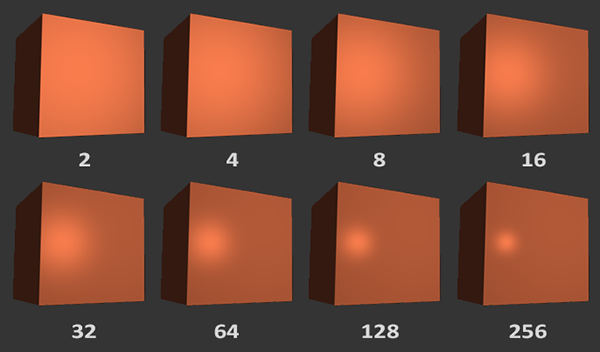
\includegraphics[height=0.30\textheight]{images/specular_shininess.png}
        \end{center}
    \end{itemize}
    \vfill{}
    {\footnotesize{Images sourced from \url{learnopengl.com/Lighting/Basic-Lighting}}}
\end{frame}

\begin{frame}[fragile]{Lighting Maps}
    \begin{itemize}
        \item Use textures to provide object colour per fragment.
        \item Use textures to specify which areas of an object give specular reflections
        \begin{center}
            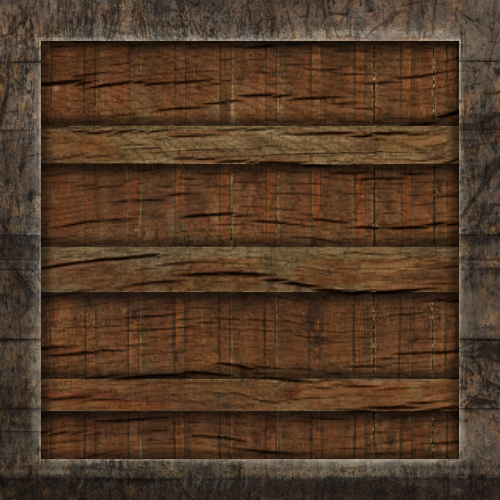
\includegraphics[height=0.30\textheight]{images/container_diffuse.png}
            
\includegraphics[height=0.30\textheight]{images/container_specular.png}
        \end{center}
        \item Use a single uniform to provide material properties per object
\footnotesize{
\begin{minted}{glsl}
    struct Material {
        sampler2D diffuse;
        sampler2D specular;
        float shininess;
    };
    in vec2 texture_coordinates;
    uniform Material material;
\end{minted}
}
        \item Use the equations as before, but sample the appropriate texture to get {\color{blue}\verb"object_colour"}.
    \end{itemize}
    \vfill{}
    {\footnotesize{Images sourced from \url{learnopengl.com/Lighting/Basic-Lighting}}}
\end{frame}

\begin{frame}[fragile]{Types of Light}
    \begin{itemize}
        \item Directional: Light source is very far away. When the light reaches the object 
            light rays are basically parallel to each other.
        \item Point Light: A nearby light that illuminates equally in all directions.
        \item Spot Light: A nearby light that illuminates in a single direction.
        \item Attentuation: Intensity of a light drops off over distance. A common formula for 
            attentuation is
            \[F_{att} = \frac{1}{K_{c} + K_{l}d + K_{q}d^{2}}\]
        \item Smoothing: Spotlight intensity fades smoothly outwards
        \[I = \frac{\cos\left(\theta\right) - \cos\left(\gamma\right)}{\cos\left(\phi\right) - \cos\left(\gamma\right)}\]
    \end{itemize}
\end{frame}

\begin{frame}[fragile]{Types of Light}
    \begin{itemize}
        \item Directional:
\footnotesize{
\begin{minted}{glsl}
    struct DirectionalLight {
        vec3 direction;

        vec3 ambient;
        vec3 diffuse;
        vec3 specular;
    };
    uniform DirectionalLight sun;
\end{minted}
}
        \item Point Light:
\footnotesize{
\begin{minted}{glsl}
    struct PointLight {
        vec3 position;

        vec3 ambient;
        vec3 diffuse;
        vec3 specular;

        float Kc;
        float Kl;
        float Kq;
    };
    uniform PointLight ceiling_light;
\end{minted}
}
    \end{itemize}
\end{frame}

\begin{frame}[fragile]{Types of Light}
    \begin{itemize}
        \item Spot Light:
\footnotesize{
\begin{minted}{glsl}
    struct SpotLight {
        vec3 position;
        vec3 direction;
        
        vec3 ambient;
        vec3 diffuse;
        vec3 specular;

        float Kc;
        float Kl;
        float Kq;

        float phi;
        float gamma;
    };
    uniform SpotLight torch;
\end{minted}
}
    \end{itemize}
\end{frame}

\end{document}
